\chapter{Mass Balance}

The body $\Bc$ is treated as a continuum, being the topological image of a domain. The mass distribution is, for now, left unspecified. In continuum mechanics, primary interest lies in mass distributions that are absolutely continuous with respect to volume.

Let $\Pi\subset\Omega$ a part of $\Omega$; here and henceforth we denote by $\Pi_t=\fb_t(\Pi)$ the image of $\Pi$ under the motion $\fb_t$. We write $\rho_{\rm ref}(\xb)>0$ for the referential mass density at the  point $\xb$  in the referential region $\Omega$ identifying the body, so that
\begin{equation}
	\int_{\Pi}\rho_{\rm ref}(\xb)\,\dd v_{\rm ref}
\end{equation}
is the mass of the region $\Pi$; we have specified the integration $\dd v_{\rm ref}$ to stress that it concerns the referential configuration.

Analogously we can introduce the current mass density $\rho(\yb,t)$ at $\yb\in\Pi_t$, so that
\begin{equation}
	\int_{\Pi_t}\rho(\yb,t)\dd v_{\rm cur}
\end{equation}
represents the mass of the region $\Pi_t$ occupied at time $t$. 

Balance of mass is the requirement that
\begin{equation}
	\int_{\Pi}\rho_{\rm ref}(\yb)\,\dd v_{\rm ref}=\int_{\Pi_t}\rho(\yb,t)\dd v_{\rm cur}
\end{equation}
for every region. The right hand side only depends on time, and then
\begin{equation}\label{bm}
	\left( \int_{\Pi_t}  \rho(\yb,t)\dd v_{\rm cur}\right)^{\dotb}=0
\end{equation}

We recall that
\begin{equation}
	\dd v_{\rm cur}=(\det\Fb)\,\dd v_{\rm ref}.
\end{equation}
We now need to state how to perform the time derivative on \eqref{bm}. Let $\varphi$ a  field given in the current representation. We have that
\begin{equation}
	\begin{aligned}
		\left( \int_{\Pi_t}  \varphi\dd v_{\rm cur}\right)^{\dotb}&=\left( \int_{\Pi}(\det\Fb)\varphi  \dd v_{\rm ref} \right)^{\dotb}\\
		&=\int_{\Pi}(\det\Fb)^{\dotb}\varphi+\dot{\varphi}(\det\Fb).
	\end{aligned}
\end{equation}
To go further we need some algebra. In particular, we need the following relation:
\begin{equation}\label{devdet}
	\partial_{\Ab}(\det\Ab)=\Ab^*
\end{equation}
and  the fact that $\operatorname{tr}{(\Ab\Bb)}=\Ab\cdot\Bb^\top$. With this, we find 
\begin{equation}
	(\det\Fb)^{\dotb}=\partial_{\Fb}(\det\Fb)\cdot\dot{\Fb}=\Fb^*\cdot\dot{\Fb}=(\det\Fb)\Fb^{-\top}\cdot\dot{\Fb}=(\det\Fb)\operatorname{tr}(\dot{\Fb}\Fb^{-1})=(\det\Fb)\operatorname{tr}\Lb=(\det\Fb)\dive\vb,
\end{equation}
whence 
\begin{equation}
	(\det\Fb)^{\dotb}=(\det\Fb)\dive \vb
\end{equation}
holds true. We therefore  conclude that
\begin{equation}
	\begin{aligned}
		\left( \int_{\Pi_t}  \varphi\dd v_{\rm cur}\right)^{\dotb}&=\int_{\Pi}(\dot{\varphi}+\varphi\dive\vb)(\det\Fb)\,\dd v_{\rm ref},
	\end{aligned}
\end{equation}
whence we get the 
\begin{definition}
\textit{\textbf{Reynolds' transport theorem}}
\begin{equation}\label{reyn}
	\begin{aligned}
		\left( \int_{\Pi_t}  \varphi\dd v_{\rm cur}\right)^{\dotb}=\int_{\Pi_t}(\dot{\varphi}+\varphi\dive\vb)\dd v_{\rm cur}.
	\end{aligned}
\end{equation}
\end{definition}
With this, \eqref{bm} reads
\begin{equation}
	\int_{\Pi_t}(\dot{\rho}+\rho\dive\vb)\dd v_{\rm cur}=0
\end{equation}
$\forall\,\Pi_t$; this quantification allows to determine the:
\begin{definition}
 \textit{\textbf{Local mass balance}}
\begin{equation}\label{masbal}
	\dot{\rho}+\rho\dive\vb=0.
\end{equation}
\end{definition}

The first term represents the rate of increase of mass, which  must be compensated by the net mass flux out of the volume (second term). To understand this, consider a small fixed control volume in space; the idea is that mass can enter or leave this volume due to the motion of the material --- that is, due to the velocity field $\vb$.

Now $\dive\vb$ measures how much the velocity field is ``spreading out'' or ``converging'' at a point, so it is the rate of volumetric expansion; if $\dive\vb>0$, then the volume at that point is expanding, so material is moving away from the point --- suggesting mass is leaving the control volume;  if $\dive\vb<0$, the volume is shrinking --- mass is entering. The quantity  $\rho \dive \vb$  gives the net rate at which mass flows out of an infinitesimal volume due to the expansion or contraction of the material.

\begin{remark}
In order to prove \eqref{devdet}, for $f(\Ab)$ a scalar-valued function of a second order $\Ab$, let us define its directional derivative in direction $\Hb\in\Lin$ as
\begin{equation}
\partial_\Ab f(\Ab)\cdot \Hb=\left.\frac{\dd}{\dd \varepsilon}f(\Ab+\varepsilon\Hb)\right|_{\varepsilon=0}.
\end{equation}
Let $f(\Ab)=\det\Ab$. Assume that $\Ab$ is invertible; then
\begin{equation}
	\Ab+\varepsilon\Hb=\Ab(\Ib+\varepsilon\Ab^{-1}\Hb),
\end{equation}
which is easily proved:
\begin{equation}
\Ab(\Ib+\varepsilon\Ab^{-1}\Hb)=\Ab+\varepsilon\Ab\Ab^{-1}\Hb=\Ab+\varepsilon\Hb.
\end{equation}
Therefore
\begin{equation}
	\det(\Ab+\varepsilon\Hb)=\det \Big(\Ab(\Ib+\varepsilon\Ab^{-1}\Hb)  \Big)=\det\Ab \, \det(\Ib+\varepsilon\Ab^{-1}\Hb),
\end{equation}
where we have made use of the Binet theorem, stating that $\det(\Ab\Bb)=\det\Ab\,\det\Bb$, for all $\Ab,\Bb\in\Lin$.

To determine $\det(\Ib+\varepsilon\Ab^{-1}\Hb)$ for $\varepsilon$ small, we notice that, for $\Bb \in\Lin$ the eigenvalues of $\Ib+\varepsilon\Bb$ are $1+\varepsilon\lambda_i$, being $\lambda_i$ the eigenvalues of $\Bb$ (this is due to the fact that $\Bb$ and $\Ib+\varepsilon\Bb$ are simultaneously triangularizable.). Therefore
\begin{equation}
	\det(\Ib+\varepsilon\Bb)=\prod_{i_1}^3(1+\varepsilon\lambda_i)=1+\varepsilon\sum_{i=1}^3\lambda_i+o(\varepsilon)=1+\varepsilon\operatorname{tr}\Bb+o(\varepsilon).
\end{equation}
Therefore, for $\varepsilon$ small, we can write
\begin{equation}
\det(\Ib+\varepsilon\Ab^{-1}\Hb)=1+\varepsilon\operatorname{tr}(\Ab^{-1}\Hb)=1+\varepsilon\Ab^{-\top}\cdot\Hb,
\end{equation}
and then
\begin{equation}
		\det(\Ab+\varepsilon\Hb)=\det(\Ab)+\varepsilon(\det\Ab)\Ab^{-\top}\cdot\Hb.
		\end{equation}

Therefore
\begin{equation}
(\partial_\Ab \det\Ab)\cdot \Hb=\left.\frac{\dd}{\dd \varepsilon}\det(\Ab+\varepsilon\Hb)\right|_{\varepsilon=0}=(\det\Ab)\Ab^{-\top}\cdot\Hb,
\end{equation}
which allows to conclude that 
\begin{equation}
	\partial_\Ab \det\Ab=(\det\Ab)\Ab^{-\top}.
\end{equation}

\end{remark}


\chapter{Force and Moment Balance}


Once a configuration $\Omega$ and a deformation $\fb(\Omega)$ are given, we address the problem of modeling the mechanical interactions that accompany them, both between parts of $\Omega$ and between $\Omega$ and the surrounding environment.

\section{Force Systems}

The simplest types of mechanical interactions are described by \textit{forces}. Over time, various concepts of \textit{force systems} have been developed with the goal of abstracting from experience and thus reflecting in a model a set of salient features of the actions on the body and the environment under consideration, both separately and when they come into contact.

The world around us offers examples of \textit{surface} actions on a body, such as the action of the wind on a sail, and \textit{volume} actions at a distance, such as gravity. The creation of a concept of a force system that efficiently accounts for these surface-contact and volume-distance interactions, as well as the creation of the corresponding notion of stress, is essentially due to \textsc{Leonhard Euler} (1707--1783) and \textsc{Augustin-Louis Cauchy} (1789--1857).

%\section{Force Systems}
Given a configuration $\widetilde{\Omega}=\fb(\Omega)$, a (Cauchy) force system formally consists of two fields:
\begin{itemize}
	\item the \textit{distance forces} $\bb(\yb)$ acting in $\widetilde\Omega$;
	\item the \textit{contact forces} $\sb(\yb)$, acting on the boundary of $\widetilde\Omega$.
\end{itemize}
The distance forces have the physical dimensions of force per unit volume, which is why they are sometimes called volume forces; the contact forces have the physical dimensions of force per unit surface area.

Given a configuration $\widetilde{\Omega}$, we define the \textit{resultant} of the forces acting in $\widetilde{\Omega}$ as
\begin{definition}
	\begin{equation}
		\rb(\widetilde{\Omega}) = \int_{\widetilde{\Omega}} \bb(\yb) + \int_{\partial\widetilde{\Omega}} \sb(\yb).
	\end{equation}
\end{definition}
We also introduce the \textit{resultant moment} with respect to the point $\yb_0$ as
\begin{definition}
	\begin{equation}
		\mb_{\yb_0}(\widetilde{\Omega}) = \int_{\widetilde{\Omega}} (\yb - \yb_0) \times \bb(\yb) + \int_{\partial\widetilde{\Omega}} (\yb - \yb_0) \times \sb(\yb).
	\end{equation}
\end{definition}


\section{Internal Actions: Stress}

The characterization of internal actions qualifies the type of continuous model being introduced; we will limit our discussion to Cauchy's model.

Crucial in the description of continuous bodies \textit{à la} Cauchy is the concept of internal action (or contact interaction). The idea, dating back to Euler, is to consider a part of the set $\widetilde{\Omega}$ and recognize that it exchanges interactions with the complementary part, which need to be characterized. This characterization specifically qualifies the class of continuous bodies we consider. In this discussion, we will only address the so-called \textit{Cauchy continua}, although this does not exhaust the class of models available for characterizing contact interactions.

Given a configuration $\widetilde{\Omega}$, we imagine separating the region in question into two parts through an orientable surface $\Sigma$, with normal $\nb$; we denote by $\widetilde{\Omega}^-$ the part that has the outward normal $\nb$ in $\widetilde{\Omega} \cap \Sigma$ and by $\widetilde{\Omega}^+=\widetilde{\Omega}\setminus\widetilde{\Omega}^-$. We fix a point $\yb$ in $\widetilde{\Omega} \cap \Sigma$. The part $\widetilde{\Omega}^-$ exchanges internal actions with $\widetilde{\Omega}^+$ through $\yb$, in the form of contact interactions, which need to be characterized.

To do this, consider a ball $B(\yb, \varepsilon)$ of radius $\varepsilon$ for $\yb$, and evaluate the resultant and the resultant moment of the forces that the region $\widetilde{\Omega}^+$ exerts on $\widetilde{\Omega}^-$ through the surface $\Sigma \cap  B(\yb,\varepsilon)$:
\begin{equation}
	\rb\big(\yb, \Sigma\cap B(\yb,\varepsilon)\big), \qquad \mb_\yb\big(\yb, \Sigma\cap B(\yb,\varepsilon)\big).
\end{equation}

\begin{figure}
	\centering
	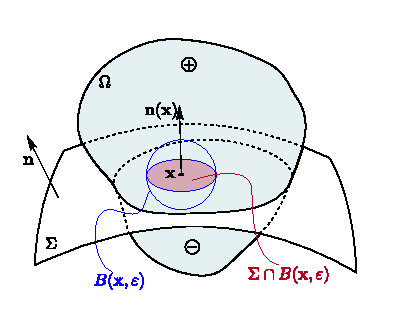
\includegraphics[scale=1.2]{figure/equilibrio/eulero3d}
	\caption{}
	\label{fig:eulero3d}
\end{figure}

Assume, according to the so-called \textit{Cauchy postulate}, that for every $\yb \in \Sigma$ there exists a $\tb(\yb; \Sigma)$ such that
\begin{definition}
	\begin{equation}
		\lim_{\varepsilon\to 0}\frac{\rb\big(\yb, \Sigma\cap B(\yb,\varepsilon)\big)}{A\big( \Sigma\cap B(\yb,\varepsilon)}=\tb(\yb, \Sigma)
	\end{equation}
\end{definition}
and
\begin{definition}
	\begin{equation}
		\lim_{\varepsilon\to 0}\frac{\mb_\yb\big(\yb, \Sigma\cap B(\yb,\varepsilon)\big)}{A\big(\yb, \Sigma\cap B(\yb,\varepsilon)}=\mathbf{0},
	\end{equation}
\end{definition}
where $A\big(\Sigma\cap B(\yb,\varepsilon)$ is the area of the surface $\Sigma\cap B(\yb,\varepsilon)$.

The field $\tb(\yb;\Sigma)$ is called the \textit{stress} and is thus the surface density of the resultant actions that the region $\widetilde{\Omega}^+$ exerts on the region $\widetilde{\Omega}^-$ through the surface $\Sigma$ at $\yb$. The density of the resultant moment is instead assumed to be zero. This choice characterizes \textit{Cauchy continua}. There exist models in which the contact interaction is not reduced to stress, but is more complex, as the density of the resultant moment is assumed to be non-zero as well; these models are commonly referred to as \textit{polar continua}.

It is important to observe that stress depends not only on the point but also on the cutting surface. We will demonstrate that:
\begin{itemize}
	\item $\tb$ depends only on the normal $\nb$ to $\Sigma$ at $\yb$ and not on all the geometric characteristics of the cutting surface (\textit{Hamel-Noll Theorem}\footnote{This theorem, in most textbooks, is considered a postulate, often called the \textit{Cauchy postulate}. From a historical point of view, it is correct, as Cauchy did not prove it, but assumed it as a given. However, the result is a simple consequence of Euler's axioms, as shown partially by Hamel and Noll.});
	\item $\tb$ depends linearly on the normal $\nb$ (\textit{Cauchy Theorem}).
\end{itemize}


\subsection{Euler's Axiom}
Let us consider a region $\Pi \subset \widetilde{\Omega}$, whose boundary $\partial\Pi$ is composed of an external part
\begin{equation}
	\partial\Pi_e \coloneqq \partial\Pi \cap \partial \widetilde{\Omega}
\end{equation}
and an internal part
\begin{equation}
	\partial\Pi_i \coloneqq \partial\Pi \setminus \partial\Pi_e.
\end{equation}

\begin{center}
	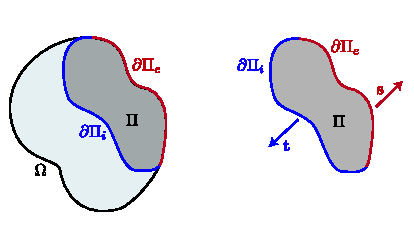
\includegraphics[scale=1.2]{figure/equilibrio/parti}
\end{center}

As stated, the resultant of the forces acting on $\bar\Pi$ is
\begin{equation}
	\rb(\Pi) = \int_{\Pi} \bb + \int_{\partial \Pi_e} \sb + \int_{\partial\Pi_i} \tb(\cdot; \partial\Pi_i),
\end{equation}
while the resultant moment with respect to the pole $\yb_0$ is
\begin{equation}
	\mb_{\yb_0}(\Pi) = \int_{\Pi} (\yb - \yb_0) \times \bb + \int_{\partial \Pi_e} (\yb - \yb_0) \times \sb + \int_{\partial \Pi_i} (\yb - \yb_0) \times \tb(\cdot; \partial\Pi_i).
\end{equation}
We assume the validity of the so-called 
\begin{definition}
	\textit{\textbf{Euler's Axiom}}. The configuration $\widetilde{\Omega}$, under the action of the volume forces $\bb$, surface forces $\sb$, and stresses $\tb$, is a configuration of equilibrium if
	\begin{equation}\label{EulAx}
		\rb(\Pi) = \mathbf{0}, \qquad \mb_{\yb_0}(\Pi) = \mathbf{0}
	\end{equation}
	for every $\Pi \subset \widetilde{\Omega}$ and for every $\yb_0$. 
\end{definition}




The body forces splits into two parts:
\begin{itemize}
	\item \textit{inertial}
	\begin{equation}
		\bb^{\rm (in)}=-\rho\dot{\vb};
	\end{equation}
	\item \textit{non-inertial}
	\begin{equation}
		\bb^{\rm (ni)}=\bb-\bb^{\rm (in)},
	\end{equation}
\end{itemize}
where the former is to be intended as a constitutive prescription. The Euler axioms then yield the \textit{balance of linear and angular momentum}:
\begin{equation}
	\rb^{\rm (ni)}(\Pi)=\dot{\lb}(\Pi), \qquad \mb_o^{\rm (ni)}(\Pi)=\dot\ab(\Pi), \quad \forall\,\Pi,
\end{equation}
where 
\begin{equation}
	\lb(\Pi):=\int_{\Pi}\rho\vb
\end{equation}
is the \textit{linear momentum} and 
\begin{equation}
	\ab(\Pi):=\int_{\Pi}\yb\times\rho\vb
\end{equation}
is the \textit{angular momentum}, and
\begin{equation}
	\rb^{\rm (ni)}(\Pi):=\int_{\partial\Pi}\tb(\nb)+\int_{\Pi}\bb^{\rm (ni)}, \qquad \mb_o^{\rm (ni)}(\Pi):=\int_{\partial\Pi}\yb\times\tb(\nb)+\int_{\Pi}\yb\times\bb^{\rm (ni)}.
\end{equation}

\begin{remark}
Given any rigid velocity field 
\begin{equation}
	\wb(\yb,t)=\wb_o(t)+\omegab(t)\times\yb
\end{equation}
and any current region $\Pi$, we define the \textit{power expended on $\Pi$ over the rigid velocity field} $\wb$
\begin{equation}
	\Wc_{\rm rig}(\Pc,\wb):=\int_{\partial\Pc}\tb(\nb)\cdot\wb+\int_{\Pi}\bb\cdot\wb.
\end{equation}
This notion has an interesting and important consequence. Since
\begin{equation}
	\begin{aligned}
		\Wc_{\rm rig}(\Pc,\wb)&=\left(\int_{\partial\Pi}\tb(\nb) + \int_{\Pi}\bb \right)\cdot \wb_o+\int_{\partial\Pi}\tb(\nb)\cdot\omegab_o\times\yb+\int_{\Pi}\bb\cdot \omegab_o\times\yb\\
		&=\rb(\Pi)\cdot\wb_o+\mb_o(\Pi)\cdot\omegab_o,
	\end{aligned}
\end{equation}
we can conclude that \textit{a system of forces is balanced if and only if the power  expended on each part $\Pi$ over a rigid velocity field vanishes}.
\end{remark}

Starting from Euler's axiom, which expresses a condition of global equilibrium, we will derive pointwise conditions. In particular, we will use the following 

\begin{definition}
	\textit{\textbf{Localization Lemma}}. If $B(\yb_0, \varepsilon) \coloneqq \{\yb : |\yb - \yb_0| \leq \varepsilon \}$ is the ball of radius $\varepsilon$ centered at $\yb_0$ with volume $V\big(B(\yb_0, \varepsilon)\big)$, $\yb_0 \in \Vc$, and $\gb$ is a continuous function in a neighborhood of $\yb_0$, then
\begin{equation}\label{lemma3}
	\lim_{\varepsilon \to 0}\frac{1}{V\big(B(\yb_0, \varepsilon)\big)}\int_{B(\yb_0, \varepsilon)} \gb (\yb) \, \dd \yb = \gb(\yb_0).
\end{equation}
\end{definition}

We will use this lemma to prove the Hamel-Noll theorem and the Cauchy theorem.

%\begin{remark}
%	We prove the localization lemma. 
%	Starting from the given expression:
%	\[
%	\frac{1}{V(B(\yb_0, \varepsilon))} \int_{B(\yb_0, \varepsilon)} \gb(\yb) \, \dd \yb.
%	\]
%	Since \( \gb \) is continuous at \( \yb_0 \), we can express \( \gb(\yb) \) as:
%	\[
%	\gb(\yb) = \gb(\yb_0) + (\gb(\yb) - \gb(\yb_0)).
%	\]
%	Substituting this expression into the integral, we get:
%	\[
%	\begin{aligned}
%		\frac{1}{V(B(\yb_0, \varepsilon))} \int_{B(\yb_0, \varepsilon)} \gb(\yb) \, \dd \yb = &\frac{1}{V(B(\yb_0, \varepsilon))} \int_{B(\yb_0, \varepsilon)} \gb(\yb_0) \, \dd \yb \\
%		&+ \frac{1}{V(B(\yb_0, \varepsilon))} \int_{B(\yb_0, \varepsilon)} (\gb(\yb) - \gb(\yb_0)) \, \dd \yb.
%	\end{aligned}
%	\]
%	The first term is easy to compute:
%	\[
%	\frac{1}{V(B(\yb_0, \varepsilon))} \int_{B(\yb_0, \varepsilon)} \gb(\yb_0) \, \dd \yb = \frac{1}{V(B(\yb_0, \varepsilon))} \cdot V(B(\yb_0, \varepsilon)) \cdot \gb(\yb_0) = \gb(\yb_0).
%	\]
%	Now consider the second term:
%	\[
%	\frac{1}{V(B(\yb_0, \varepsilon))} \int_{B(\yb_0, \varepsilon)} (\gb(\yb) - \gb(\yb_0)) \, \dd \yb.
%	\]
%	Since \( \gb \) is continuous at \( \yb_0 \), for every \( \delta > 0 \), there exists an \( \varepsilon > 0 \) sufficiently small such that:
%	\[
%	|\gb(\yb) - \gb(\yb_0)| < \delta \quad \text{for every} \quad \yb \in B(\yb_0, \varepsilon).
%	\]
%	This allows us to estimate the second term:
%	\[
%	\left| \frac{1}{V(B(\yb_0, \varepsilon))} \int_{B(\yb_0, \varepsilon)} (\gb(\yb) - \gb(\yb_0)) \, \dd \yb \right| \leq \frac{1}{V(B(\yb_0, \varepsilon))} \int_{B(\yb_0, \varepsilon)} |\gb(\yb) - \gb(\yb_0)| \, \dd \yb.
%	\]
%	Since \( |\gb(\yb) - \gb(\yb_0)| < \delta \) for every \( \yb \in B(\yb_0, \varepsilon) \), we get:
%	\[
%	\frac{1}{V(B(\yb_0, \varepsilon))} \int_{B(\yb_0, \varepsilon)} |\gb(\yb) - \gb(\yb_0)| \, \dd \yb \leq \delta.
%	\]
%	
%	Since \( \delta \) can be made arbitrarily small by choosing \( \varepsilon \) sufficiently small, we conclude that:
%	\[
%	\lim_{\varepsilon \to 0} \frac{1}{V(B(\yb_0, \varepsilon))} \int_{B(\yb_0, \varepsilon)} (\gb(\yb) - \gb(\yb_0)) \, \dd \yb = 0.
%	\]
%	
%	Combining the results, we get:
%	\[
%	\lim_{\varepsilon \to 0} \frac{1}{V(B(\yb_0, \varepsilon))} \int_{B(\yb_0, \varepsilon)} \gb(\yb) \, \dd \yb = \gb(\yb_0).
%	\]
%	
%	Therefore, the theorem is proved.
%\end{remark}


\subsection{The Hamel-Noll Theorem}
We state the 
\begin{definition}
	\textbf{\textit{Hamel-Noll Theorem}} Given two surfaces $\Sigma$ and $\hat\Sigma$ that have at least one common point $\yb_0 \in \Sigma \cap \hat{\Sigma} \subset \widetilde{\Omega}$ and share the same normal vector $\nb$ at $\yb_0$, then for an equilibrium configuration $\Omega$ under the action of $\{\bb, \sb, \tb\}$, we have
	\begin{equation}\label{HN0}
		\tb(\yb_0;\Sigma) = \tb(\yb_0;\hat\Sigma).
	\end{equation}
\end{definition}

In other words, the stress depends only on the normal vector; we can therefore define
\begin{equation}
	\tb(\yb_0, \nb) \coloneqq \tb(\yb_0; \Sigma) = \tb(\yb_0; \hat\Sigma).
\end{equation}

We now prove the theorem. The surface $\Sigma$ divides the region $\Omega$ into two parts, $\Omega^-$ and $\Omega^+$; similarly, the surface $\hat{\Sigma}$ divides the region $\Omega$ into two parts, $\hat\Omega^-$ and $\hat\Omega^+$. Consider the semi-cylinder $C_\varepsilon$ with an axis passing through $\yb_0$, a circular base of radius $\varepsilon$ orthogonal to $\nb$, and at a distance of $\varepsilon^2$ from $\nb$, contained in $\Omega^- \cap \hat{\Omega}^-$.

We define
\begin{equation}
	P_{\varepsilon} \coloneqq C_\varepsilon \cap \Omega^-, \qquad \hat{P}_{\varepsilon} \coloneqq C_\varepsilon \cap \hat\Omega^-
\end{equation}
as the parts of the semi-cylinder contained in $\Omega^-$ and $\hat\Omega^-$. 

\begin{center}
	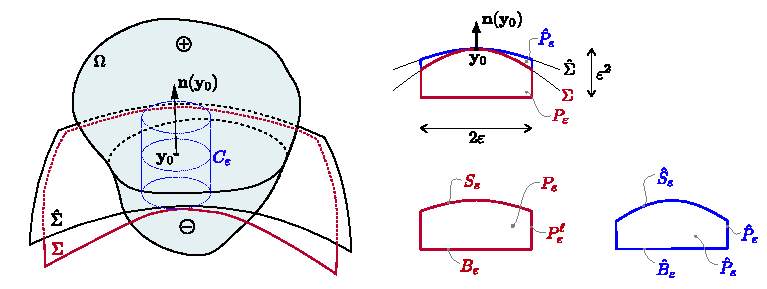
\includegraphics[scale=1.2]{figure/equilibrio/hamelnoll}
\end{center}

We write the translational equilibrium of $P_{\varepsilon}$:
\begin{equation}\label{rHN}
	\rb(P_\varepsilon) = \int_{P_\varepsilon} \bb + \int_{B_\varepsilon} \tb(\cdot; B_\varepsilon) + \int_{P^\ell_\varepsilon} \tb(\cdot; P^\ell_\varepsilon) + \int_{S_\varepsilon} \tb(\cdot; \Sigma) = \mathbf{0},
\end{equation}
where $B_\varepsilon$ is the base and $P^\ell_\varepsilon$ is the lateral surface of $P_\varepsilon$, while $S_\varepsilon \coloneqq P_\varepsilon \cap \Sigma$ is the "upper base," obtained by intersecting $P_{\varepsilon}$ with the surface $\Sigma$. We observe that the volume $V(P_\varepsilon)$ is of order $O(\varepsilon^4)$, the area $A(P_\varepsilon^\ell)$ is of order $O(\varepsilon^3)$, the area $A(B_\varepsilon)$ is of order $O(\varepsilon^2)$, and the area $A(S_\varepsilon)$ is of order $\varepsilon^2$.

We divide \eqref{rHN} by $A(S_\varepsilon)$ and rewrite it to apply the localization lemma:
\begin{equation}
	\begin{aligned}
		&\frac{V(P_\varepsilon)}{A(S_\varepsilon)} \, \frac{1}{V(P_\varepsilon)} \int_{P_\varepsilon} \bb +
		\frac{A(B_\varepsilon)}{A(S_\varepsilon)} \frac{1}{A(B_\varepsilon)} \int_{B_\varepsilon} \tb(\cdot; B_\varepsilon) + \frac{A(P^\ell_\varepsilon)}{A(S_\varepsilon)} \int_{P^\ell_\varepsilon} \tb(\cdot; P^\ell_\varepsilon) \\
		& + \frac{1}{A(S_\varepsilon)} \int_{S_\varepsilon} \tb(\cdot; \Sigma) = \mathbf{0}.
	\end{aligned}
\end{equation}
As $\varepsilon$ tends to zero,
\begin{equation}
	\frac{V(P_\varepsilon)}{A(S_\varepsilon)} \to 0, \quad \frac{A(P^\ell_\varepsilon)}{A(S_\varepsilon)} \to 0, \quad \frac{A(B_\varepsilon)}{A(S_\varepsilon)} \to 1, \quad \frac{1}{A(S_\varepsilon)} \int_{S_\varepsilon} \tb(\cdot; S_\varepsilon) \to \tb(\yb_0; \Sigma)
\end{equation}
and thus
\begin{equation}\label{HN1}
	\tb(\yb_0; \Sigma) + \lim_{\varepsilon \to 0} \frac{1}{A(B_\varepsilon)} \int_{B_\varepsilon} \tb(\cdot; B_\varepsilon) = \mathbf{0}.
\end{equation}

Now, requiring that the equilibrium condition holds for $\hat P_\varepsilon$, we get
\begin{equation}
	\rb(\hat P_\varepsilon) = \int_{\hat P_\varepsilon} \bb + \int_{B_\varepsilon} \tb(\cdot; B_\varepsilon) + \int_{\hat P^\ell_\varepsilon} \tb(\cdot; \hat P^\ell_\varepsilon) + \int_{\hat S_\varepsilon} \tb(\cdot; \hat{\Sigma}) = \mathbf{0}.
\end{equation}
Proceeding as for $P_\varepsilon$, we obtain
\begin{equation}\label{HN2}
	\tb(\yb_0; \hat\Sigma) + \lim_{\varepsilon \to 0} \frac{1}{A(B_\varepsilon)} \int_{B_\varepsilon} \tb(\cdot; B_\varepsilon) = \mathbf{0}.
\end{equation}
From \eqref{HN1} and \eqref{HN2}, we immediately obtain \eqref{HN0}.



\subsection{The Cauchy Theorem}

Let’s immediately state the theorem:

\begin{definition}
	Let \(\Omega\) be an equilibrium configuration for \(\{\bb, \sb, \tb\}\). Then the stress depends linearly on the normal; in particular, there exists a tensor field \(\Tb \,:\, \Omega \to \Lin\), called the \textit{Cauchy stress tensor}, such that
	\[
	\tb(\yb_0, \nb) = \Tb(\yb_0) \nb,
	\]
	for every \(\yb_0 \in \Omega\) and every unit vector \(\nb\).
\end{definition}

The theorem is a milestone in continuum mechanics, as Cauchy himself proudly recognized. The proof, published in 1823, elegantly uses a construction based on certain geometric properties of the tetrahedron, which we will recall shortly. One undeniable value of this proof is that it is constructive: not only does it produce an existence result for the stress tensor, but it also provides an explicit representation of it.

Next, we will first recall some geometric properties of the tetrahedron, which are essential for the proof, and then establish a preparatory result, usually referred to as the \textit{Cauchy Lemma}.

\subsubsection{Geometry of the Tetrahedron} 
Consider a tetrahedron with three mutually orthogonal faces with area \(A_i\) and external normal \(\eb_i\), while the inclined face has area \(A\) and external normal \(\nb\), with \(\nb \cdot \eb_i > 0\) for \(i = 1, 2, 3\). We want to prove the following property:
\begin{equation}\label{Ai}
	\frac{A_i}{A} = \nb \cdot \eb_i.
\end{equation}
Let \(\vb_i\) denote the three vectors that go from the origin to the intersection point \(P_i\) of the oblique plane with the axes parallel to \(\eb_i\).

\begin{center}
	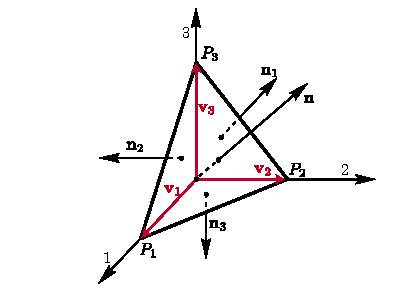
\includegraphics[scale=1.2]{figure/equilibrio/tetraedro}
\end{center}

Observe that \(\overrightarrow{P_1P_2} = \vb_2 - \vb_1\) and \(\overrightarrow{P_1P_3} = \vb_3 - \vb_1\). Then, using the properties of the vector cross product, we have
\[
\begin{aligned}
	A \nb &= \frac{1}{2} \overrightarrow{P_1P_2} \times \overrightarrow{P_1P_3} = \frac{1}{2} (\vb_1 \times \vb_3 - \vb_2 \times \vb_1 - \vb_1 \times \vb_3) \\
	&= A_1 \eb_1 + A_2 \eb_2 + A_3 \eb_3,
\end{aligned}
\]
from which equation \eqref{Ai} follows.

\subsubsection{Cauchy’s Lemma}
We state Cauchy’s lemma:

\begin{definition}
	The stress \(\tb(\yb_0, \nb)\) is an odd function of \(\nb\), i.e.
	\begin{equation}\label{lemmaC}
		\tb\big(\yb_0, \nb(\yb_0)\big) = -\tb\big(\yb_0, -\nb(\yb_0)\big).
	\end{equation}
\end{definition}

The physical interpretation is clear: at a point \(\yb_0\), the stress recorded on a plane with normal \(\nb\) is equal and opposite to the stress on the plane with normal \(-\nb\). This is nothing but the formalization of the \textit{action and reaction principle} in this context.

To prove this, we use an argument similar to the one used to prove the Hamel-Noll theorem. Suppose the region \(\Omega\) is separated into two parts by a surface \(\Sigma\) with normal \(\nb\) at \(\yb_0\). Consider a semi-cylinder \(C_\varepsilon\), with radius \(\varepsilon\), base \(B_\varepsilon\) situated at a distance \(\varepsilon^2\) from \(\yb_0\) and axis parallel to \(\nb\). We require that the part \(P_\varepsilon\) is in equilibrium:
\begin{equation}
	\rb(P_\varepsilon) = \int_{P_\varepsilon} \bb + \int_{B_\varepsilon} \tb(\cdot; -\nb) + \int_{P^\ell_\varepsilon} \tb(\cdot; \mb) + \int_{S_\varepsilon} \tb(\cdot; \nb) = \mathbf{0},
\end{equation}
where \(P^\ell_\varepsilon\) is the lateral surface of \(P_\varepsilon\), with outward normal \(\mb\), and \(S_\varepsilon = P_\varepsilon \cap \Sigma\). Dividing by the area \(A(S_\varepsilon)\) and taking the limit as \(\varepsilon\) goes to zero, using the usual localization lemma, we obtain
\begin{equation}
	\tb(\yb_0, -\nb(\yb_0)) + \tb(\yb_0, \nb(\yb_0)) = \mathbf{0},
\end{equation}
which gives the expected result.

\subsubsection{The Tetrahedron Argument}
Now, let’s proceed with the proof of the Cauchy theorem using the tetrahedron argument. Consider an internal part \(\Tc_\varepsilon\) of \(\Omega\), shaped like a tetrahedron with three edges passing through \(\yb_0\) and parallel to a fixed arbitrary Cartesian coordinate system. Let \(\varepsilon\) be the distance from \(\yb_0\) to the oblique face \(S_\varepsilon\), with normal \(\nb\), and area \(A(S_\varepsilon)\); the other faces \(S^i_\varepsilon\) have area \(A(S^i_\varepsilon)\) and outward normal \(-\eb_i\).

We impose equilibrium on the tetrahedron:
\begin{equation}
	\int_{\Tc_\varepsilon} \bb + \int_{S_\varepsilon} \tb(\cdot, \nb) + \sum_{i=1}^{3} \int_{S_\varepsilon^i} \tb(\cdot, -\eb_i) = \mathbf{0}.
\end{equation}
Dividing by \(A(S_\varepsilon)\), we get
\begin{equation}
	\frac{V(\Tc_\varepsilon)}{A(S_\varepsilon)} \frac{1}{V(\Tc_\varepsilon)} \int_{\Tc_\varepsilon} \bb + \frac{1}{A(S_\varepsilon)} \int_{S_\varepsilon} \tb(\cdot, \nb) + \sum_{i=1}^{3} \frac{A(S^i_\varepsilon)}{A(S_\varepsilon)} \frac{1}{A(S^i_\varepsilon)} \int_{S_\varepsilon^i} \tb(\cdot, -\eb_i) = \mathbf{0}.
\end{equation}
Using the result \eqref{Ai} and taking \(\varepsilon \to 0\), since \(V(\Tc_\varepsilon) = O(\varepsilon^3)\) and \(A(S_\varepsilon) = O(\varepsilon^2)\), we get
\[
\tb(\yb_0, \nb) = -\sum_{i=1}^{3} (\nb \cdot \eb_i) \tb(\yb_0, -\eb_i).
\]
Now, by applying Cauchy’s lemma \eqref{lemmaC}, we conclude that
\[
\tb(\yb_0, \nb) = \sum_{i=1}^{3} (\nb \cdot \eb_i) \tb(\yb_0, \eb_i) = \left(\sum_{i=1}^{3} \tb(\yb_0, \eb_i) \otimes \eb_i \right) \nb.
\]

We define
\begin{definition}
	\begin{equation}\label{Tb}
		\Tb(\yb_0) \coloneqq \sum_{i=1}^{3} \tb(\yb_0, \eb_i) \otimes \eb_i,
	\end{equation}
\end{definition}
so that we can write
\begin{definition}
	\begin{equation}\label{tTn}
		\tb(\yb_0, \nb) = \Tb(\yb_0) \nb,
	\end{equation}
\end{definition}
which shows that the stress vector at \(\yb_0\) relative to the orientation defined by \(\nb\) is obtained by applying the linear operator \(\Tb(\yb_0)\) to \(\nb\). The tensor field \(\Tb\) represents the so-called \textit{Cauchy stress tensor}. As anticipated, the proof is constructive: \(\Tb\) is explicitly represented by equation \eqref{Tb}, which reveals that to construct the stress tensor at a point, it is necessary to know the stress vector on three mutually orthogonal planes; once this is known, the stress on any plane can be determined using equation \eqref{tTn}.

\newpage
Once a basis \(\{\eb_i\}\) is chosen, we can determine the components of \(\Tb\):
\begin{equation}
	T_{ij} = \Tb \eb_j \cdot \eb_i = \tb(\cdot, \eb_i) \cdot \eb_i = t_i(\cdot, \eb_j).
\end{equation}
Thus, \(T_{ij}\) represents the \(i\)-th component of the stress on a plane with normal \(\eb_j\).

\begin{center}
	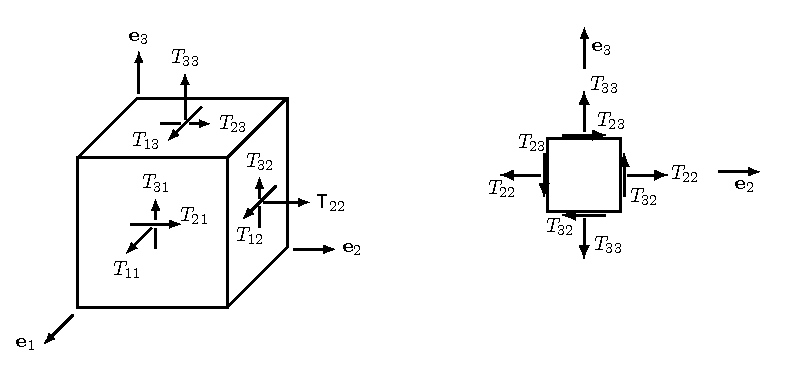
\includegraphics[scale=1]{figure/equilibrio/componenti_tensione}
\end{center}

\begin{exercise}
	At point \(\yb_0\), the stress on three planes with normal \(\eb_i\) \((i=1,2,3)\) is known:
	\begin{equation}
		\begin{aligned}
			&\tb_1(\yb_0, \eb_1) = \alpha \eb_1 - \beta \eb_3, \\
			&\tb_2(\yb_0, \eb_2) = \gamma \eb_2+\beta\eb_3, \\
			&\tb_3(\yb_0, \eb_3) = \beta (-\eb_1+\eb_2) + \gamma \eb_3.
		\end{aligned}
	\end{equation}
	Determine the stress on the plane with normal \(\nb = \frac{1}{\sqrt{2}}(\eb_1 + \eb_2)\).
	\begin{svolgimento}
		Given the stress on three planes at \(\yb_0\), the definition of \(\Tb\) allows us to determine the stress tensor:
		\begin{equation}
			\begin{aligned}
				&\Tb(\yb_0) = \alpha (\eb_1 \otimes \eb_1) + \gamma (\eb_2 \otimes \eb_2+\eb_3 \otimes \eb_3) - \beta (\eb_ 1\otimes \eb_3+ \eb_3 \otimes \eb_1-\eb_ 2\otimes \eb_3-\eb_ 3\otimes \eb_2) \\
				&\tb(\yb_0, \nb) = \Tb(\yb_0) \nb = \frac{1}{\sqrt{2}}(\alpha\eb_1+\gamma\eb_2).
			\end{aligned}
			\end{equation}
		\end{svolgimento}	
		\end{exercise}




\section{Pointwise Equilibrium Equations}
\subsection{Cauchy’s Relation for Interior Points}
Consider initially a point \(\yb_0\) inside \(\Omega\), an equilibrium configuration for \(\{\bb, \sb, \tb\}\). Let \(B(\yb_0, \varepsilon)\) be the ball centered at \(\yb_0\), with radius \(\varepsilon\), chosen small enough to ensure that \(B(\yb_0, \varepsilon) \subset \Omega\). For this ball, Euler's axiom holds:
\begin{equation}
	\int_{B(\yb_0,\varepsilon)} \bb + \int_{\partial B(\yb_0,\varepsilon)} \tb(\cdot, \nb) = \mathbf{0},
\end{equation}
or, invoking Cauchy's theorem:
\begin{equation}
	\int_{B(\yb_0, \varepsilon)} \bb + \int_{\partial B(\yb_0, \varepsilon)} \Tb \nb = \mathbf{0}.
\end{equation}
Using the divergence theorem, we obtain:
\begin{equation}\label{eq1int}
	\int_{B(\yb_0, \varepsilon)} \bb + \dive \Tb = \mathbf{0}.
\end{equation}
Dividing by \(V(B(\yb_0, \varepsilon))\) and sending \(\varepsilon\) to zero, applying the localization lemma \eqref{lemma3}, we get:
\begin{definition}
	\begin{equation}\label{bDiv}
		\bb(\yb_0) + \dive \Tb(\yb_0) = \mathbf{0},
	\end{equation}
\end{definition}
for every point \(\yb_0\) inside \(\Omega\).

%Choosing a basis \(\{\eb_i\}\), equation \eqref{bDiv} can be written componentwise:
%\begin{definition}
%	\begin{equation}
%		\begin{cases}
%			b_1 + \dfrac{\partial T_{11}}{\partial y_1} + \dfrac{\partial T_{12}}{\partial y_2} + \dfrac{\partial T_{13}}{\partial y_3} = 0,\\[.3cm]
%			b_2 + \dfrac{\partial T_{21}}{\partial y_1} + \dfrac{\partial T_{22}}{\partial y_2} + \dfrac{\partial T_{23}}{\partial y_3} = 0,\\[.3cm]
%			b_3 + \dfrac{\partial T_{31}}{\partial y_1} + \dfrac{\partial T_{32}}{\partial y_2} + \dfrac{\partial T_{33}}{\partial y_3} = 0.
%		\end{cases}
%	\end{equation}
%\end{definition}

\subsection{Cauchy’s Relation for Boundary Points}
Now, let \(\yb_0\) be a point belonging to the boundary \(\partial\Omega\). Consider the semi-cylinder \(C_\varepsilon\) with an axis passing through \(\yb_0\) and parallel to \(\nb(\yb_0)\), with a base of radius \(\varepsilon\) that is at a distance \(\varepsilon^2\) from \(\yb_0\). Let \(P_\varepsilon = \Omega \cap C_\varepsilon\). The translational equilibrium of \(P_\varepsilon\) requires that:
\begin{equation}
	\int_{P_\varepsilon} \bb + \int_{S_\varepsilon} \sb + \int_{B_\varepsilon} \Tb(-\nb) + \int_{P_\varepsilon^\ell} \Tb \mb,
\end{equation}
where \(B_\varepsilon\) is the base of \(P_\varepsilon\), \(P_\varepsilon^\ell\) is the lateral surface with outward normal \(\mb\), and \(S_\varepsilon = \partial P_\varepsilon \cap \partial \Omega\). Dividing by \(A(B_\varepsilon)\) and sending \(\varepsilon\) to zero, we obtain, using the usual argument:
\begin{equation}
	\sb(\yb_0) - \Tb(\yb_0) \nb(\yb_0) = \mathbf{0},
\end{equation}
or
\begin{definition}
	\begin{equation}\label{Tns}
		\Tb(\yb_0) \nb(\yb_0) = \sb(\yb_0)
	\end{equation}
\end{definition}
for every \(\yb_0 \in \partial \Omega\). The stress field \(\Tb(\yb_0)\) is understood as the extension to the boundary of \(\Tb\), which is actually defined on the open set \(\Omega\). Equation \eqref{Tns} establishes that, on the boundary of \(\Omega\), the stress vector is equal to the contact force exerted by the external environment on the body.

\subsection{The Symmetry of the Stress Tensor}
Up until now, we have not used the second equilibrium condition \eqref{EulAx}, which holds when a system of forces is in equilibrium. Let us now apply it to a ball \( B(\yb_0, \varepsilon) \) of radius \(\varepsilon\) centered at \(\yb_0\), using Cauchy's theorem:
\begin{equation}
	\int_{ B(\yb_0, \varepsilon)} \yb \times \bb + \int_{ \partial B(\yb_0, \varepsilon)} \yb \times \sb = \int_{ B(\yb_0, \varepsilon)} \yb \times \bb + \int_{ \partial B(\yb_0, \varepsilon)} \yb \times \Tb \nb = \mathbf{0}.
\end{equation}
Let \(\wb \in \Vc\) be a constant vector, and \(\Wb \in \Skw\) such that \(\wb \times \ab = \Wb \ab\) for any \(\ab \in \Vc\); trivially, we have
\begin{equation}
	\int_{ B(\yb_0, \varepsilon)} \wb \cdot \yb \times \bb + \int_{ \partial B(\yb_0, \varepsilon)} \wb \cdot \yb \times \Tb \nb = 0.
\end{equation}
Since \(\wb \cdot \yb \times \bb = \bb \cdot \wb \times \yb = \bb \cdot \Wb \yb\) and \(\wb \cdot \yb \times \Tb \nb = \Tb \nb \cdot \Wb \yb\), we can write:
\begin{equation}
	\int_{ B(\yb_0, \varepsilon)} \bb \cdot \Wb \yb + \int_{ \partial B(\yb_0, \varepsilon)} \nb \cdot \Tb^\top \Wb \yb = \int_{ B(\yb_0, \varepsilon)} \dive(\Tb^\top \Wb \yb) = 0,
\end{equation}
where we used the divergence theorem for the last equality. Using the identity
\begin{equation}
	\dive (\Ab \gb) = (\dive \Ab^\top) \cdot \gb + \Ab^\top \cdot \grad \gb,
\end{equation}
which is valid for any \(\Ab \in \Lin\) and \(\gb \in \Vc\), we can write
\begin{equation}
	\dive(\Tb^\top \Wb \yb) = (\dive \Tb) \cdot \Wb \yb + \Tb \cdot \Wb,
\end{equation}
and thus
\begin{equation}
	\int_{ B(\yb_0, \varepsilon)} (\bb + \dive \Tb) \cdot \Wb \yb + \Tb \cdot \Wb = 0.
\end{equation}
Note that, due to \eqref{eq1int}, the first term is zero. Dividing by the volume of the ball and taking the limit \(\varepsilon \to 0\), we then obtain
\begin{equation}
	\Tb(\yb_0) \cdot \Wb = 0.
\end{equation}
Given the arbitrariness of \(\Wb \in \Skw\), we conclude that
\begin{definition}
	\begin{equation}
		\Tb(\yb_0) \in \Sym.
	\end{equation}
\end{definition}
Thus, the stress field associated with a balanced system of forces must have \textit{symmetric} values.

\vspace{.2cm}
In conclusion, the Cauchy stress tensor associated with an equilibrium configuration for a set \(\{\bb, \sb, \tb\}\) must satisfy the following conditions:
\begin{definition}
	\begin{equation}\label{pstat}
		\begin{cases}
			\begin{array}{ll}
				\dive \Tb + \bb = \mathbf{0}, & \qquad \text{in} \; \Omega \\
				\Tb = \Tb^\top, & \qquad \text{in} \; \Omega \\
				\Tb \nb = \sb, & \qquad \text{on} \; \partial \Omega,
			\end{array}
		\end{cases}
	\end{equation}
\end{definition}

Given a configuration \(\Omega\) and a system of external forces \(\{\bb, \sb\}\), a stress field \(\Tb\) on \(\Omega\) is said to solve the corresponding \textit{static problem} if the conditions \eqref{pstat} are satisfied. The system \eqref{pstat} forms a set of 3 partial differential equations with 6 unknowns, the components of the stress tensor; in general, this problem does not admit a unique solution.


\begin{comment}
\begin{exercise}
	The stress tensor in the cube $\Omega=(-1,1)\times(-1,1)\times(-1,1)$ has a representative matrix
	\begin{equation}
		[\Tb]=\left[\begin{array}{ccc}
			\sigma y_2 y_3 & \sigma y_2^2 & \sigma(y_1-y_3) \\
			\sigma y_2^2 & \sigma y_2 & 0 \\
			\sigma(y_1-y_3) & 0 & \sigma y_3
		\end{array}\right].
	\end{equation}
	Knowing that the cube is in equilibrium, determine the applied volume and surface forces.
	\begin{svolgimento}
		Using \eqref{bDiv}, we immediately obtain
		\begin{equation}
			\begin{aligned}
				&    -b_1=(\dive \Tb)_1=T_{1j,j}=T_{11,1}+T_{12,2}+T_{13,3}=\sigma(2y_2-1), \\
				&-b_2=(\dive \Tb)_2=T_{2j,j}=T_{21,1}+T_{22,2}+T_{23,3}=\sigma, \\
				&-b_3=(\dive \Tb)_3=T_{3j,j}=T_{31,1}+T_{32,2}+T_{33,3}=2\sigma
			\end{aligned}
		\end{equation}
		or
		\begin{equation}
			\bb = \sigma\Big(  (1-2y_2)\eb_1+\eb_2+2\eb_3 \Big).
		\end{equation}
		To determine the applied surface forces on the face with normal $\eb$, we need to evaluate $\Tb$ on the plane $y_1=1$ and then observe its action on $\nb =\eb_1$:
		\begin{equation}
			[\Tb(1,y_2,y_3)]=\left[\begin{array}{ccc}
				\sigma y_2 y_3 & \sigma y_2^2 & \sigma(1-y_3) \\
				\sigma y_2^2 & \sigma y_2 & 0 \\
				\sigma(1-y_3) & 0 & \sigma y_3
			\end{array}\right]
			\left[\begin{array}{c}
				1 \\
				0 \\
				0
			\end{array}\right] = \sigma
			\left[\begin{array}{c}
				y_2 y_3 \\
				y_2^2 \\
				1 - y_3
			\end{array}\right],
		\end{equation}
		and so on for the other faces.
	\end{svolgimento}
\end{exercise}


\begin{exercise}
	Let a Cartesian coordinate system $(y_1, y_2, y_3)$ be given, and consider the cylindrical coordinate system $(\rho, \theta, z)$, with $y_1=\rho \cos \theta$, $y_2=\rho \sin \theta$, $y_3=z$, and the associated orthonormal basis $\{\eb_\rho, \eb_\theta, \eb_z\}$,
	\begin{equation}
		\eb_\rho=\cos\theta\eb_1+\sin\theta\eb_2, \quad \eb_\theta=-\sin\theta\eb_1+\cos\theta\eb_2, \quad \eb_z=\eb_3.
	\end{equation}
	The hollow cylinder
	\begin{equation}
		(R-\delta)<\rho< R, \quad 0\leq\theta<2\pi, \quad -L/2< z< L/2
	\end{equation}
	\begin{center}
		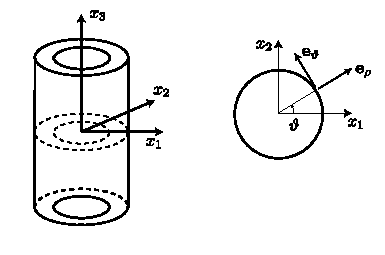
\includegraphics[scale=1.2]{figure/equilibrio/esempio13d}
	\end{center}
	is subjected to the stress
	\begin{equation}
		\Tb=2\sigma \eb_\vartheta\otimes \eb_\vartheta+\sigma \eb_z \otimes \eb_z +\frac{\tau}{R}\rho (\eb_\vartheta\otimes\eb_z+\eb_z\otimes\eb_\vartheta).
	\end{equation}
	\begin{enumerate}
		\item Write the Cartesian components of the stress field $\tb$ on the transverse section with outward normal $\eb_3$ for the origin.
		\item On the longitudinal section of the cylinder with outward normal $\eb_1$ for the origin, calculate the Cartesian components of the resultant vector $\rb$ of the stresses and the resultant moment vector $\mb_0$ with respect to the origin.
	\end{enumerate}
	\begin{svolgimento}
		\begin{enumerate}
			\item The stress on the face with normal $\eb_3$ is found using Cauchy's theorem
			\begin{equation}
				\Tb \eb_z=\sigma \eb_z +\frac{\tau}{R}\rho \eb_\vartheta=\frac{\tau}{R}(-y_2\eb_1+y_1\eb_2)+\sigma \eb_3.
			\end{equation}
			\item 
			It is necessary to determine the stress on the surfaces $\Sc_1$ and $\Sc_2$, with normal $\eb_1$.
			\begin{center}
				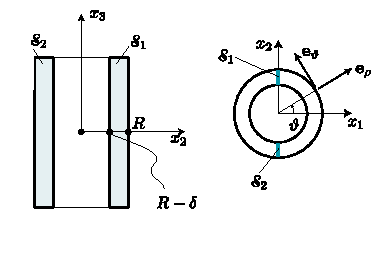
\includegraphics[scale=1.2]{figure/equilibrio/esempio13d_1}
			\end{center}
			We find that
			\begin{equation}
				\Tb \eb_1=2\sigma \sin^2\vartheta \eb_1-2\sigma\sin\vartheta\cos\vartheta\eb_2-\frac{\tau}{R}\rho \sin\vartheta\eb_3.
			\end{equation}
			On $\Sc_1$ we have $\vartheta=\pi/2$, so
			\begin{equation}
				\tb_1=\Tb \eb_1|_{\vartheta=\pi/2}=2\sigma\eb_1-\frac{\tau}{R}\rho \eb_3,
			\end{equation}
			while on $\Sc_2$ we have $\vartheta=-\pi/2$, so
			\begin{equation}
				\tb_2=\Tb \eb_1|_{\vartheta=-\pi/2}=2\sigma\eb_1+\frac{\tau}{R}\rho \eb_3.
			\end{equation}
			The resultant is then
			\begin{equation}
				\rb=\int_{-L/2}^{L/2}\int_{R-\delta}^{R}\tb_{1}+\tb_{2}=4\sigma \delta L \eb_1.
			\end{equation}
			To calculate the resultant moment with respect to the origin, we need to determine the lever arm: the position of the generic point is
			\begin{equation}
				\yb=\rho\cos\vartheta\eb_1+\rho \sin\vartheta\eb_2+y_3\eb_{3},
			\end{equation}
			on $\Sc_1$ we have
			\begin{equation}
				\yb_1 = \rho\, \eb_2+y_3\,\eb_3,
			\end{equation}
			while on $\Sc_1$ we have
			\begin{equation}
				\yb_2= -\rho\, \eb_2+y_3\,\eb_3.
			\end{equation}
			The resultant moment is then
			\begin{equation}
				\mb_0=\int_{-L/2}^{L/2}\int_{R-\delta}^R\yb_1\times \tb_1+\yb_2\times \tb_2=-\frac23 \frac{\tau}{R}(R^3-(R-\delta)^3)\,\eb_1.
			\end{equation}
		\end{enumerate}
	\end{svolgimento}
\end{exercise}

\begin{exercise}
	Let $\bar\Tb$ be the average stress in a configuration $\Omega$ subjected to volume forces $\bb$ and contact forces $\sb$ in equilibrium. Using the divergence theorem, prove that
	\begin{equation}
		\bar\Tb=\frac{1}{\textrm{vol}(\Omega)}\left( \int_{\Omega}\yb\otimes\bb+\int_{\partial\Omega}\yb\otimes\sb \right),
	\end{equation}
	where $\yb$ is the generic point in $\Omega$.
	\begin{svolgimento}
		First, observe that
		\begin{equation}
			\int_{\partial\Omega}\yb\otimes \sb=\int_{\partial\Omega}\yb\otimes \Tb \nb,
		\end{equation}
		on which we apply the divergence theorem. Working component-wise. Given a vector $\ab\in \Vc$ and a tensor $\Ab \in \Lin$,
		\begin{equation}
			(\ab \otimes \Ab \nb)_{ij}=a_i A_{jk}n_k
		\end{equation}
		and thus, by the divergence theorem
		\begin{equation}
			\int_{\partial\Omega}a_i A_{jk}n_k=\int_{\Omega}(a_i A_{jk}),_{k}.
		\end{equation}
		We have that 
		\begin{equation}
			(a_i A_{jk}),_{k}=a_{i,k}A_{jk}+a_i A_{jk,k}=\big((\grad \ab)\, \Ab^\top\big)_{ij}+(\ab \otimes \dive \Ab)_{ij}
		\end{equation}
		and thus
		\begin{equation}
			\int_{\partial\Omega}\ab \otimes \Ab \nb =\int_{\Omega}(\grad \ab)\, \Ab^\top+\ab \otimes \dive \Ab.
		\end{equation}
		Using this general result with $\ab=\yb$ and $\Ab =\Tb$:
		\begin{equation}
			\int_{\partial\Omega}\yb \otimes \Tb \nb =\int_{\Omega}(\grad \yb)\, \Tb^\top+\yb \otimes \dive \Ab=\int_{\Omega}\Tb -\yb \otimes \bb,
		\end{equation}
		from which it follows immediately that
		\begin{equation}
			\int_{\Omega}\yb \otimes \bb +\int_{\partial \Omega}\yb \otimes\sb=\int_{\Omega}\Tb,
		\end{equation}
		and thus the desired result is immediately obtained.
	\end{svolgimento}
\end{exercise}
\end{comment}

%
%\section{Principal Stresses}
%The stress vector recorded on a plane with normal vector $\nb$ generally has two components: one parallel to $\nb$
%\begin{equation}
%	\sigmab\coloneqq\sigma\nb \quad\sigma\coloneqq \tb(\nb) \cdot \nb
%\end{equation}
%called the \textit{normal stress}, and one perpendicular to $\nb$
%\begin{equation}
%	\taub\coloneqq \tb(\nb) -\sigmab.
%\end{equation}
%called the \textit{shear stress}. One may ask whether there are orientations for which the stress is purely normal. To answer this question, we need to solve the problem
%\begin{equation}\label{autov}
%	\tb(\nb)=\sigmab \quad  \Longleftrightarrow\quad \Tb \nb =\sigma \nb.
%\end{equation}
%Equation \eqref{autov}$_2$ shows that to answer our question, we need to solve an \textit{eigenvalue problem}. Since $\Tb$ is a symmetric tensor, we can appeal to the spectral theorem to conclude that its eigenvalues are all real and the eigenvectors are mutually orthogonal. Therefore, there exist three orientations, orthogonal to each other, where the stress is purely normal. The stress tensor can then be given the following \textit{spectral representation}:
%\begin{definition}
%	\begin{equation}
%		\mathbf{T}=\sum_{i=1}^3\lambda_i\mathbf{n}_i\otimes\mathbf{n}_i
%	\end{equation}
%\end{definition}
%where $\lambda_i$ are the (real) eigenvalues of $\Tb$ and $\nb_i$ are the corresponding (orthonormal) eigenvectors. The eigenvalues are called \textit{principal stresses}, and the eigenvectors are called \textit{principal directions}. We conventionally number the principal stresses as follows:
%\begin{equation}
%	\lambda_1\leq\lambda_2\leq\lambda_3.
%\end{equation}
%Thus, $\lambda_3$ is the maximum normal stress, and $\lambda_1$ is the minimum.
%
%The envelope of the principal directions defines three families of mutually orthogonal curves, known as \textit{isostatic lines}. Along these curves, the stresses are purely normal, and therefore, the material is simply compressed or stretched along these directions. Furthermore, these lines represent the points of maximum tension and compression.
%
%\begin{figure}[h!]
%	\centering
%	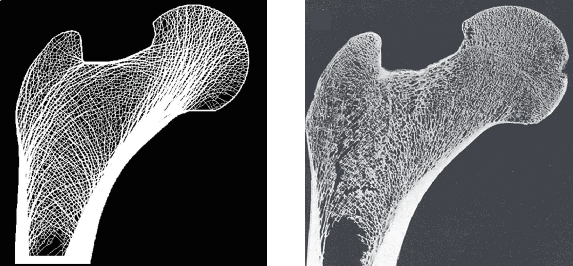
\includegraphics[width=0.8\linewidth]{figure/cinematica/osso_direzprinc}
%	\caption{Trabecular structure in a proximal femur, determined through a model (left) and actual (right). The arrangement of the trabeculae follows the isostatic lines. (Adapted from M. Huo, S. He, Y. Zhang, Y. Feng, J. Lu, Simulation on bone remodeling with stochastic nature of adult and elderly using topology optimization algorithm, Journal of Biomechanics, Volume 136, 2022.)}
%	\label{fig:ossodirezprinc}
%\end{figure}


%
%
%Nature optimizes the use of material by constructing structures that have the shape, size, and strength needed with the least possible mass. A clear example of this principle is observed in \textit{long bones}, such as the femur or humerus, where the trabeculae are arranged along the isostatic lines.
%
%The arrangement of the trabeculae along the isostatic lines had been observed long before Cauchy formally described the stress state. However, more recently, it has been shown that many living organisms can continuously model and remodel themselves in response to signals derived from the local stress state. These signals are generated by the external loads the organism must support. Taking the long bones again as an example, this adaptation process is made possible by the combined action of \textit{osteoclasts}, which break down bone tissue, and \textit{osteoblasts}, which rebuild it.
%

\section{External power, kinetic energy, inertial power}\label{kinetic}
We define \textit{external (non-inertial) power} expended on $\Pi$ as 
\begin{equation}
	\Wc^{(\rm ni)}(\Pi):=\int_{\partial\Pi}\Tb\nb\cdot\vb+\int_{\Pi}\bb^{(\rm ni)}\cdot\vb.
\end{equation}

The field
\begin{equation}
	\frac{1}{2} \rho |\vb|^2
\end{equation}
is the \textit{kinetic energy} measured per unit volume in the deformed body; hence
\begin{equation}
	K(\Pi):=\int_{\Pi}\frac{1}{2} \rho |\vb|^2
\end{equation} 
is the \textit{kinetic energy} of $\Pi$.

There is a basic relation between the kinetic-energy rate and the power expended by the inertial force $\bb^{(\rm in)}$:
\begin{equation}
	\begin{aligned}
		\left( \int_{\Pi}\frac{1}{2} \rho |\vb|^2 \right)^{\dotb}&= \frac{1}{2}\int_{\Pi}\left( \rho|\vb^2| \right)^{\dotb}+\rho|\vb|^2\dive\vb=\frac{1}{2}\int_{\Pi}\dot{\rho}|\vb|^2+\rho(|\vb|^2)^{\dotb}+\rho|\vb|^2\dive\vb\\
		&=\frac{1}{2}\int_{\Pi}\rho(|\vb|^2)^{\dotb}+|\vb|^2(\dot{\rho}+\rho\dive\vb)=\int_{\Pi}\rho\dot\vb\cdot\vb=\int_{\Pi}-\bb^{(\rm in)}\cdot\vb,
	\end{aligned}
\end{equation}
where we have made use of the mass balance; we conclude that
\begin{equation}
	\Wc^{(\rm in)}(\Pi)=-\dot K(\Pi), \qquad \Wc^{(\rm in)}(\Pi):=\int_{\Pi}\bb^{(\rm in)}\cdot\vb
\end{equation}
which means that the inertial power expenditure is balanced by the negative kinetic-energy rate of $\Pi$. As a consequence
\begin{equation}\label{bpow}
	\int_{\Pi}\bb\cdot\vb=\int_{\Pi}\bb^{(\rm ni)}\cdot\vb-\dot{\Kc}(\Pi).
\end{equation}

As to the power of contact force, we may use the divergence theorem, the identity \eqref{divid}, and the local balance equation to obtain
\begin{equation}\label{tpow}
	\int_{\partial\Pi}\Tb\nb\cdot\vb=\int_{\Pi}(\dive\Tb)\cdot\vb+\Tb\cdot\grad\vb=\int_{\Pi}\Tb\cdot\grad\vb-\bb\cdot\vb;
\end{equation}
by the symmetry of $\Tb$, we have that
\begin{equation}\label{strpow}
	\Tb\cdot\grad\vb=\Tb\cdot\Db.
\end{equation}
The right side of this latter relation establishes that the stretching $\Db$ as the appropriate power-conjugate variable for the Cauchy stress $\Tb$, and we say that $\Tb$ is power conjugate to $\Db$. The field
$$
\Tb\cdot\Db
$$
represents the power expended within $\Pi$, measured per unit volume, ad is referred as the \textit{stress power}; the integral 
\begin{equation}
	\Wc^{(\rm int)}=\int_{\Pi}\Tb\cdot\Db
\end{equation}
represents the net power expended within $\Pi$ and is referred as the internal power. Combining \eqref{bpow}, \eqref{tpow}, and \eqref{strpow}, we arrive at the power balance:
\begin{definition}
\begin{equation}\label{powerbal}
	\int_{\partial\Pi}\Tb\nb\cdot\vb+\int_{\Pi}\bb\cdot\vb=\int_{\Pi}\Tb\cdot\Db,
\end{equation}
\end{definition}
or, equivalently
\begin{equation}
	\int_{\partial\Pi}\Tb\nb\cdot\vb+\int_{\Pi}\bb^{(\rm ni)}\cdot\vb=\int_{\Pi}\Tb\cdot\Db+\dot{K}(\Pi),
\end{equation}
or rather
\begin{equation}
	\Wc^{(\rm ni)}(\Pi)=\Wc^{(\rm int)}(\Pi)+\dot{K}(\Pi).
\end{equation}
If we define as external power
\begin{equation}
	\Wc^{\rm (ext)}(\Pi)=\Wc^{(\rm ni)}(\Pi)+\Wc^{(\rm in)}(\Pi),
\end{equation}
we get
\begin{equation}
	\Wc^{\rm (ext)}(\Pi)=\Wc^{(\rm int)}(\Pi).
\end{equation}


\section{Referential form for the force balance}
When working with solids, the use a current description can be problematic; for this reason we now reformulate the basic laws in a referential setting.

Let us denote by $\Pb$ the stress measured per unit area in the reference body; it is called \textit{Piola stress}. For $\Pi \subset \Omega$, the following relation holds true:
\begin{equation}
	\int_{\fb(\partial\Pi)}\Tb\nb\dd a_{\rm cur}=\int_{\partial\Pi}\Pb\nb_{\rm ref}\dd a_{\rm ref};
\end{equation}
from \eqref{nanson} we deduce that

\begin{equation}
	\nb\dd a_{\rm cur}=(\det\Fb)\Fb^{-\top}\nb_{\rm ref}\dd a_{\rm ref}
\end{equation}

and then
\begin{equation}
	\int_{\partial\Pi}(\det\Fb)\Tb\Fb^{-\top}\nb_{\rm ref}\dd a_{\rm ref}=\int_{\partial\Pi}\Pb\nb_{\rm ref}\dd a_{\rm ref},
\end{equation}
whence
\begin{definition}
\begin{equation}\label{Pio}
	\Pb=(\det\Fb)\Tb\Fb^{-\top}.
\end{equation}
\end{definition}
The Piola stress  carries the referential vector $\nb_{\rm ref}$ to the traction $\Pb\nb_{\rm ref}$ , which is a current vector; thus, like the deformation gradient, $\Pb$ maps  the referential vector space  into the current vector space.

As to the body force, we have that
\begin{equation}
	\int_{\fb(\Pi)}\bb\dd v_{\rm cur}=\int_{\Pi}\bb_{\rm ref}\dd v_{\rm ref},
\end{equation}
whence
\begin{equation}
	\bb_{\rm ref}=(\det\Fb)\bb;
\end{equation}
it represents the  body force measured per unit volume in the reference body.

The \textit{balance of forces}, expressed referentially is then
\begin{equation}
	\int_{\partial\Pi}\Pb\nb_{\rm ref}+\int_{\Pi}\bb_{\rm ref}=\mathbf{0};
\end{equation}
on denoting by $\Div$ the referential divergence operator, it is straightforward to get the local balance of linear forces:
\begin{equation}
	\Div\Pb+\bb_{\rm ref}=\mathbf{0},
\end{equation} 
valid in the referential configuration $\Omega$
Moreover, since $\Tb=\Tb^\top$, and $\Tb=(\det\Fb)^{-1}\Pb\Fb^\top$, the balance of moments in $\Omega$ reads
\begin{equation}
	\Pb\Fb^\top=\Fb\Pb^\top.
\end{equation}


A referential version for the stress power is given by the following identity:
\begin{equation}
	\Tb\cdot\Db=\Tb\cdot\Lb=\Tb\cdot(\dot\Fb\Fb^{-1})=(\Tb\Fb^{-\top})\cdot\dot{\Fb}=(\det\Fb)^{-1}\Pb\cdot\dot{\Fb};
\end{equation}
hence
\begin{equation}\label{CaPi}
	\Tb\cdot\Db=(\det\Fb)^{-1}\Pb\cdot\dot{\Fb}.
\end{equation}
Thus
\begin{definition}
\begin{equation}
	\int_{\fb(\Pi)}\Tb\cdot\Db\dd v_{\rm cur}=\int_{\Pi}\Pb\cdot\dot{\Fb}\dd v_{\rm ref}.
\end{equation}
\end{definition}
The field $\Pb\cdot\dot{\Fb}$ represents the stress power measured per unit volume in the reference body.


\subsection{Power-conjugate pairings. Second Piola stress}
The stress power $\Tb\cdot\Db$ and $\Pb\cdot\dot{\Fb}$ are two examples of power-conjugate pairing. There is a crucial difference between $\Db$ and $\dot{\Fb}$: the former is purely a measure of the rate at which material elements stretch, while the latter carries information concerning the rates at which material elements stretch and rotate. One might therefore ask whether there are alternative referential measures of stress power in which a measure of stress is paired with a pure strain-rate.

In particular, we seek a pairing involving a measure $\Sb$ of stress that is conjugate to the time-rate $\dot{\Cb}$ of the right Cauchy-Green tensor. To determine the form of $\Sb$, we notice the following set of identities:
\begin{equation}
	\begin{aligned}
		\Tb\cdot\Db&=\frac 12 \Tb\cdot(\Lb+\Lb^\top)=\\
		&=\frac 12 \Tb\cdot(\dot{\Fb}\Fb^{-1}+\Fb^{-\top}\dot{\Fb}^\top)\\
		&=\frac 12 \Tb\cdot\Fb^{-\top}(\Fb^\top\dot{\Fb}+\dot{\Fb}^\top\Fb)\Fb^{-1}\\
		&=\frac 12 (\Fb^{-1}\Tb\Fb^{-\top})\cdot(\Fb^\top\dot{\Fb}+\dot{\Fb}^\top\Fb)\\
		&=\frac 12 (\Fb^{-1}\Tb\Fb^{-\top})\cdot\dot\Cb\\
		&=\frac 12(\det\Fb)^{-1}(\Fb^{-1}\Pb)\cdot\dot{\Cb}.
	\end{aligned}
\end{equation}
We define the \textit{second Piola stress tensor} as 
\begin{definition}
\begin{equation}
	\Sb:=\Fb^{-1}\Pb=(\det \Fb)\,\Fb^{-1}\Tb \Fb^{-\top}
\end{equation}
\end{definition}
so that
\begin{equation}
	\Tb\cdot\Db=\frac{1}{2}(\det\Fb)^{-1}\Sb\cdot\dot{\Cb}.
\end{equation}
We notice that the second Piola stress tensor is symmetric.

The Cauchy stress $\Tb$ maps $\Vcu$ into $\Vcu$; the Piola stress $\Pb$ maps $\Vr$ into $\Vcu$; the second Piola stress $\Sb$ maps $\Vr$ into $\Vr$.


In continuum mechanics, different stress tensors describe internal forces from different perspectives, depending on whether they refer to the current or reference configuration. The \emph{Cauchy stress tensor} $\Tb$ is the most physical and directly measurable one: it gives the force per unit area acting on a surface element \emph{in the deformed configuration}. That is, it tells how internal forces are transmitted across a cut in the current body. The \emph{first Piola stress tensor} \(\Pb \) represents the same actual forces, but expressed with respect to \emph{undeformed} surface elements. It thus combines current forces with reference areas, making it a mixed (and generally non-symmetric) object. Finally, the \emph{second Piola stress tensor} \( \Sb \) fully pulls the description back to the reference configuration: it expresses both forces and areas as if the body were still undeformed. This makes \(\Sb \) symmetric. In summary, \( \Tb \) lives in the deformed configuration, \(\Pb\) mixes current forces and reference areas, and \(\Sb\) lives entirely in the reference world.




\chapter{Frame indifference}\label{FI}
\section{Frame of reference}
The region $\fb_t(\Omega)$ is observed during the motion. The ambient space through which $\Omega_t$ evolves is termed the \textit{observed space}; the ambient space for the reference body is termed \textit{reference space}.

A \textit{change of frame} is defined, at each fixed time $t$, by a rotation $\Qb(t)$ and a translation $\wb(t)$ of the observed space and transforms current points to current points:
\begin{equation}\label{y+}
	\yb^+=\wb(t)+\Qb(t)\yb.
\end{equation}

We refer to $\wb(t)\in\Ecu$ as the \textit{frame translation} and $\Qb(t)\in\Rot$ as the \textit{frame rotation}. Since $\Qb\in\Rot$,
\begin{equation}
	\Qb\Qb^\top=\Ib \quad \Rightarrow\quad (\Qb\Qb^\top)^{\dotb}=\mathbf{0}, \quad \Rightarrow\quad \dot{\Qb}\Qb^\top+\Qb\dot{\Qb}^\top=\mathbf{0},
\end{equation}
and then then
\begin{equation}
	\Omegab:=\dot{\Qb}\Qb^\top\in\Skw,
\end{equation}
and it is called frame-spin; $\Omegab$ represents  the rate at which the new frame is spinning. It is worth noticing that a change of frame does not affect the reference space and then reference points and reference vectors are \textit{invariant} under changes in frame; moreover scalar fields such as the density are invariant: $\rho^+=\rho$.

\subsection{Frame-indifferent fields}
A vector field is \textit{frame-indifferent} if it simply rotates with the frame rotation:
\begin{equation}
	\gb^+=\Qb\gb.
\end{equation}
A tensor field $\Gb$ is frame indifferent if, given indifferent vector fileds $\hb$ and $\gb$, with $\gb$ arbitrary, and any change in frame,
\begin{equation}
	\hb=\Gb\gb \quad {\rm implies} \quad \hb^+=\Gb^+\gb^+.
\end{equation}
Now, if $\hb=\Gb\gb$ it follows that
\begin{equation}
	\hb^+=\Qb\hb=\Qb\Gb\gb=\Qb\Gb\Qb^\top\gb^+,
\end{equation}
where we have used the fact that $\gb=\Qb^\top\gb^+$. We then conclude that
\begin{equation}
	\Gb^+=\Qb\Gb\Qb^\top.
\end{equation}

\subsection{Transformation rules for kinematic fields}
Since $\yb=\fb(\xb,t)$ is a current point, but $\xb$ is referential, eq. \eqref{y+} implies
\begin{equation}
	\fb^+(\xb,t)=\wb(t)+\Qb(t)\, \fb(\xb,t) .
\end{equation}
On taking the gradient with respect to $\xb$, we get
\begin{equation}
	\Fb^+(\xb,t)=\Qb(t)\Fb(\xb,t).
\end{equation}
From this relation we get:
\begin{equation}
	\Cb^+=(\Fb^+)^\top\Fb^+=\Fb^\top \Qb \Qb \Fb=\Fb^\top\Fb \quad \Rightarrow \quad \Cb^+=\Cb.
\end{equation}
Then the fields $\Cb$, $\Ub$, $\Eb$ are \textit{invariant}.
On recalling that $\Rb=\Fb\Ub^{-1}$ and $\Fb^+=\Qb\Fb$, we conclude that
\begin{equation}
	\Rb^+=\Qb\Fb\Ub^{-1}=\Qb\Rb.
\end{equation}



As to the velocity gradient, we get
\begin{equation}\label{Lb+}
	\Lb^+=(\Fb^+)^{\mathop{\vcenter{\hbox{\Large$\cdot$}}}}(\Fb^+)^{-1}=(\Qb\dot\Fb+\dot\Qb\Fb)(\Fb^{-1}\Qb^{-1})=\Qb \dot\Fb\Fb^{-1}\Qb^\top+\dot\Qb\Qb^\top=\Qb\Lb\Qb^\top+\Omegab.
\end{equation}

In summary:
\begin{definition}
\begin{equation}
	\begin{aligned}
		&\Fb^+=\Qb\Fb,\\
		&\Rb^+=\Qb\Rb,\\
		&\Ub^+=\Ub,\\
		&\Cb^+=\Cb,\\
		&\Eb_{\rm G}^+=\Eb_{\rm G},\\
		&\Vb^+=\Qb\Vb\Qb^\top,\\
		&\Bb^+=\Qb\Bb\Qb^\top,\\
		& \Lb^+=\Qb\Lb\Qb^\top+\Omegab.
	\end{aligned}
\end{equation}
\end{definition}
In other words:
\begin{itemize}
	\item the tensors $\Vb$ and $\Bb$ are \textit{frame-indifferent};
	\item the tensors $\Ub$, $\Cb$, $\Eb_{\rm G}$ are \textit{invariant};
	\item the tensors $\Fb$, $\Lb$ and $\Rb$ are neither frame-indifferent nor invariant.
\end{itemize}


\section{Frame-indifference principle}
A basic principle underlying most of physics is that
\begin{itemize}
	\item \emph{physical laws be independent of the frame of reference},
\end{itemize}
which is the frame-indifference principle.

\subsection{Transformation rules for stress and body force}
We assume that the balance of forces is frame-indifferent:
\begin{equation}
	\int_{\partial\Pi_t^+}\Tb^+\nb^++\int_{\Pi_t^+}\bb^+=\mathbf{0},
\end{equation}
where $\Pi_t^+=\fb^+(\Pi,t)$ is the deformed region $\Pi_t$ as viewed with respect to the new frame. The mapping $\tb(\nb)=\Tb\nb$ carries current vectors $\nb$ to current vectors $\tb$. We assume that
\begin{equation}
	\tb^+=\Qb\tb, \quad \nb^+=\Qb\nb.
\end{equation}
It follows that
\begin{equation}
	\tb^+=\Tb^+\nb^+ \quad \Rightarrow\quad \Qb\tb=\Tb^+\Qb\nb  \quad \Rightarrow\quad \tb=(\Qb^\top\Tb^+\Qb)\nb=\Tb\nb,
\end{equation}
which allows to conclude that
\begin{definition}
	\begin{equation}
	\Tb^+=\Qb\Tb\Qb^\top;
\end{equation}
\end{definition}
then the \textit{Cauchy stress is frame indifferent}.
Since
\begin{equation}
	\int_{\partial\Pi_t^+}\Tb^+\nb^+=\int_{\partial\Pi_t}(\Qb\Tb\Qb^\top)\Qb\nb=\Qb\int_{\partial\Pi_t}\Tb\nb,
\end{equation}
we conclude that
\begin{equation}
	\int_{\Pi_t^+}\bb^+=\Qb\int_{\partial\Pi_t}\Tb\nb=\Qb\bb;
\end{equation}
thus the \textit{body force is frame indifferent}.









\chapter{Principle of Virtual Powers}\label{PPV}

In mechanics, there are two distinct ways to provide a mathematical representation of the concept of force. The first is to represent it as an \textit{applied vector}, a mathematical entity characterized by an origin, magnitude, direction, and sense. Its natural extension to continuous media leads to the definition of vector fields associated with measures, hence giving rise to `body forces', `surface forces', `forces per unit mass', and so on.

The second approach, which dates back at least to d'Alembert, is what is commonly referred to as the \textit{principle of virtual power}. This second method is in fact more natural than the first, as it mathematically formalizes what is typically done in practice to evaluate a force. For example, if one wants to assess the weight of an object, the most natural operation is to `weigh' it --- that is, to apply a velocity and gauge the effort required to do so. Our brain cannot directly perceive a force, but only the power it expends.

From a mathematical standpoint, this procedure can be described as follows: at a given instant, a virtual velocity field \( \tilde\vb \) is considered on the system \( \Pi \); the forces producing this motion are known if their \textit{virtual power} is known. More precisely --- and more abstractly --- one considers a set  of virtual velocities \( \tilde\vb \), and the forces acting on the system are said to be known if there exists a linear functional \( \mathcal{W}(\Pi)[\tilde\vb] \) whose value, for every \( \tilde\vb \), equals the virtual power produced by the forces during the motion defined by \( \tilde\vb \).

The core idea underlying this second viewpoint is that of \textit{duality}. One of its main advantages lies in the flexibility it offers in defining the space of virtual velocities, allowing for a more or less refined description of the system's motion.  It must be acknowledged that the notion of a linear functional defined on a vector space is more abstract and mathematically involved than that of a vector field, which explains why the first description of force historically prevailed, at least initially. Furthermore, when this idea first emerged, the concept of duality --- which can be seen as a precursor to the modern notions of \textit{measure} and \textit{distribution} --- had not yet been fully developed. Today, functional analysis and its applications to mechanics have provided powerful mathematical tools for the notion of duality, and since at least the mid-20th century, the use of concepts related to virtual power and duality has proven extremely fruitful in the development of field theories.


In this chapter we rederive the balance laws for force and moment. Unlike traditional treatments, we do not take these laws as starting assumptions. Instead, we show how they can be deduced from more basic premises. In the same spirit, we do not assume the validity of Cauchy’s formula $\tb(\nb)=\Tb \nb$.

\section{Principle of Virtual Power}
Our starting point is the generalized power balance \eqref{powerbal}, written in a more general form that avoids invoking Cauchy’s theorem:
\begin{equation}\label{powerbal1}
\int_{\partial \Pi}\tb(\nb)\cdot \vb+\int_\Pi \bb\cdot\vb=\int_\Pi \Tb \cdot \grad \vb.
\end{equation}
The defining feature of \eqref{powerbal1} is that it incorporates the Cauchy stress via its internal power expenditure, without assuming symmetry or frame indifference.

We reinterpret the power balance  \eqref{powerbal1} by replacing the actual velocity $\vb$ with a virtual field $\tilde{\vb}$, not connected to the real motion. Time $t$ is held fixed, so $\tilde{\vb}$  is treated as an arbitrary function, and $\Pi$ as any subregion of the deformed body $\widetilde{\Omega}$.

On denoting by
\begin{equation}
\Wc^{\rm (ext)}(\Pi)[\tilde{\vb}]=\int_{\partial \Pi}\tb(\nb)\cdot \tilde\vb+\int_\Pi \bb\cdot\tilde\vb, \qquad \Wc^{\rm (int)}(\Pi)[\tilde{\vb}]=\int_\Pi \Tb \cdot \grad \tilde\vb
\end{equation}
the esternal and internal virtual power, we rewrite  \eqref{powerbal1} in the form of a 
\begin{definition}
\textbf{Virtual Power Balance}
\begin{equation}\label{VPB}
\int_{\partial \Pi}\tb(\nb)\cdot \tilde\vb+\int_\Pi \bb\cdot\tilde\vb=\int_\Pi \Tb \cdot \grad \tilde\vb.
\end{equation}
\end{definition}

\section{Force balance, stress}
We now show that the \eqref{VPB} encapsulates the local force balance and the Cauchy theorem.   Assume that \eqref{VPB} is satisfied for all $\Pi$ and $\tilde\vb$. Then, using the divergence theorem, we get
\begin{equation}
\int_\Pi\Tb \cdot \grad \tilde\vb=\int_{\partial\Pi}\Tb\cdot\tilde\vb-\int_\Pi\dive \Tb \cdot \tilde\vb,
\end{equation}
ant then, by  \eqref{VPB},
\begin{equation}
\int_\Pi (\dive\Tb +\bb)\cdot \tilde \vb +\int_{\partial\Pi}(\tb(\nb)-\Tb\nb)\cdot \tilde \vb=0,
\end{equation}
for every choice of the field $\tilde\vb$. We appeal to the 
\begin{definition}
\textbf{Fundamental Lemma  of the Calculus of Variations}: Let $\fb$ be a continuous vector field on $\Pi$, let $\hb$ be a continuous vector field on a smooth subsurface $\Sigma$ of $\partial\Pi$, and assume that
\begin{equation}
\int_{\Pi}\fb\cdot\bm{\phi}+\int_{\Sigma}\hb\cdot\bm{\phi}=0
\end{equation}
for all continuous vector fields $\bm{\phi}$ on $\Pi$, that vanishes on $\partial\Pi\setminus\Sigma$. Then
\begin{equation}
\fb=\mathbf{0} \quad \textrm{in $\Pi$}, \qquad \hb=\mathbf{0}\quad \textrm{in $\Sigma$}.
\end{equation}
\end{definition}
This lemma, with $\Sigma=\partial\Pi$ and $\bm{\phi}=\tilde\vb$ allows to  conclude that
\begin{equation}
\dive\Tb +\bb=\mathbf{0}
\end{equation}
in $\Pi$ and 
\begin{equation}
\tb(\nb)=\Tb\nb
\end{equation}
on $\partial\Pi$. Since $\Pi$ is arbitrary, these relations must hold throughout $\widetilde{\Omega}$.


\section{Symmetry and frame-indifference}\label{symPVP}
We now show that the requirement that the internal virtual power $ \Wc^{\rm (int)}(\Pi)[\tilde{\vb}]$ be invariant under changes of frame implies that $\Tb$ is symmetric and frame-indifferent.
Assuming time is fixed and omitted, we introduce an arbitrary frame change represented by the mapping $\bm{\phi}$, which takes  points $\yb$ to $\yb^+$, in accordance with \eqref{y+}; namely,
\begin{equation}\label{yb+}
	\yb^+=\bm{\phi}(\yb)=\wb+\Qb\,\yb,
\end{equation}
with $\Qb$ the frame rotation.  To facilitate the discussion of how the internal power transforms, it is helpful to keep the spatial arguments explicit. For this reason, we express the internal power in the following way:
\begin{equation}
 \Wc^{\rm (int)}(\Pi)[\tilde{\vb}]=\int_\Pi\Tb(\yb) \cdot \grad \tilde\vb(\yb).
\end{equation}
The virtual velocity gradient $\tilde\Lb(\yb)=\grad\tilde\vb(\yb)$ transforms under the change of frame as \eqref{Lb+}:
\begin{equation}\label{L+v}
\tilde\Lb(\yb^+)=\Qb \tilde\Lb(\yb)\Qb^\top+\Omegab.
\end{equation}
The frame-indifference then requires that
\begin{equation}\label{FRIT}
\int_{\Pi}\Tb(\yb)\cdot \tilde\Lb(\yb)\,\dd v(\yb)=\int_{\Pi^+}\Tb^{+}(\yb^+)\cdot\tilde\Lb^+(\yb^+)\,\dd v(\yb^+).
\end{equation}
On using \eqref{yb+} and \eqref{L+v}, we can write the RHS as 
\begin{equation}
\int_{\Pi^+}\Tb^{+}(\yb^+)\cdot\tilde\Lb(\yb^+)\,\dd v(\yb^+)=\int_{\Pi^+}\Tb^{+}(\yb^+)\cdot\Big(  \Qb \tilde\Lb(\bm{\phi}^{-1}(\yb^+)\Qb^\top+\Omegab\Big)  \,\dd v(\yb^+).
\end{equation}
Since the Jacobian of the transformation $\bm{\phi}$ satisfies $\det\grad \bm{\phi}=\det\Qb=1$, if we change the variable of integration from $\yb^+$ to $\yb$ we find that
\begin{equation}
	\int_{\Pi^+}\Tb^{+}(\yb^+)\cdot\tilde\Lb(\yb^+)\,\dd v(\yb^+)=\int_{\Pi}\Tb^{+}(\bm{\phi}(\yb))\cdot\Big(  \Qb \tilde\Lb(\yb)\Qb^\top+\Omegab\Big)  \,\dd v(\yb).
\end{equation}
Therefore, the frame indifference requirement \eqref{FRIT} implies
\begin{equation}
	\int_{\Pi}\Tb(\yb)\cdot \tilde\Lb(\yb)\,\dd v(\yb)=\int_{\Pi}\Tb^{+}(\bm{\phi}(\yb))\cdot\Big(  \Qb \tilde\Lb(\yb)\Qb^\top+\Omegab\Big)  \,\dd v(\yb).
\end{equation}
or, equivalently, since the region $\Pi$ is arbitrary
\begin{equation}
\Tb\cdot\tilde\Lb=\Tb^+\cdot (\Qb \tilde\Lb \Qb^\top+\Omegab)=(\Qb^\top\Tb^+\Qb)\cdot\tilde\Lb+\Tb^+\cdot\Omegab,
\end{equation}
where we have suppressed arguments.

Let us consider a change of frame in which $\Qb$ is constant. We therefore have that
\begin{equation}
(\Tb-\Qb^\top\Tb^+\Qb)\cdot\tilde\Lb=0,
\end{equation}
for all choices of $\tilde\Lb$, and then
\begin{equation}
	\Tb^+=\Qb\Tb\Qb^\top.
\end{equation}
The Cauchy stress is therefore frame-indifferent. With this, we find that
\begin{equation}
\Tb^+\cdot\Omegab=0;
\end{equation}
on the other hand,  we may assume that $\Omegab$ is an arbitrary skew-symmetric tensor; thus $\Tb^+=(\Tb^+)^\top$, and then
\begin{equation}
	\Tb=\Tb^\top;
\end{equation}
the Cauchy stress is therefore symmetric.

The preceding results highlight the broad applicability of the principle of virtual power. Its significance becomes especially evident in nonclassical contexts where additional kinematical degrees of freedom are present. Notably, we will make repeated use of this principle in our discussion of plasticity.

\begin{remark}
One often finds this principle formulated \textit{erroneously} in terms of an underlying free energy, an error
arising from the observation that — in the absence of dissipation — energy minimization generally
results in partial-differential equations equivalent to those resulting from a corresponding virtual-power principle.

\end{remark}



